\documentclass[11pt]{article}

% Call the style package
%\usepackage{fun3style}

\title{HRI Project: PepperChef}
\author{Riccardo Caprari, ID number 1743168\\Emanuele Giacomini, ID number 1743995\\ \\Department of Computer, Control, and Management Engineering \\Sapienza University of Rome}
\date{Fall 2020}

\usepackage{multirow}
\usepackage{lineno, hyperref, subfig}

\usepackage{graphicx}
\graphicspath{{./img/}}

\usepackage[utf8]{inputenc}
\usepackage[english]{babel}

\usepackage{xcolor}
\usepackage{nth}
\usepackage{amsmath}
\usepackage{relsize}
\usepackage{wrapfig}
\usepackage{float}
\usepackage{listings}

\usepackage{caption}

\usepackage{csquotes}
\usepackage{float}
\usepackage{amssymb}
\usepackage{multicol}
\usepackage{ragged2e}

\usepackage[bottom=1.5in, left=1.5in, right=1.5in]{geometry}

\usepackage{indentfirst}
\usepackage{etoolbox}
\patchcmd{\thebibliography}{\section*{\refname}}{}{}{}

\setlength{\parindent}{0em}
\setlength{\parskip}{1em}

\DeclareMathOperator{\EX}{\mathbb{E}}% expected value

\begin{document}


\maketitle

\vspace{6px}

\openup -3ex
\tableofcontents
\openup 3ex

\newpage
\textbf{Contributions}

We hereby declare that the project work entitled \textbf{PepperChef} is developed in equal contribution by Riccardo Caprari and Emanuele Giacomini. In particular, Riccardo took care of the processes involved in the user-tablet interaction with the use of MODIM APIs, video elaboration/commenting and half of this report. Emanuele, instead, took care of the main app running on Pepper, handling the gesturing, part of dialog and actions, plus the other half of the report.


\section{Introduction}\label{cha:intro}

PepperChef is a project based on the use of Pepper robot by SoftBank Robotics. We focus our work on the development of an application that suits the actions and feelings of Pepper in a kitchen environment. The purpose is, in fact, to have a robot that is capable of assisting people in their daily lives, in particular when preparing meals. This study takes into account the emotional and social aspects of people, trying to create a bond of friendship in those moments of the day in which persons may be alone and concentrated on something to prepare. PepperChef could be one solution to reinvent the art of cooking in the kitchen, guiding people in the preparation while making it easier and less tiring.

Loneliness, which can often be linked to depression, is a very deep state of mind. Sometimes it comes to help us and make us think about a situation or how to solve a problem. Some other times these feelings can seriously hurt our mood. We can resume PepperChef in two important aspects: a kitchen supervisor for recipes preparation and a companion robot to reduce loneliness and bad moods. This last side highlights the importance of solutions like PepperChef, trying to solve problems which deeply affects people and their lives. What we want to obtain is not only a virtual chef ready to teach delightful recipes but also a real friend, which is anyway constrained by the actual robot capabilities.

The development of the application takes care of Pepper's dialog and interaction processes with humans. We bring a work that let the final user learn some cooking recipes of various difficulties in a soft and enjoyable way. People can interact with PepperChef using their voice in a real scenario, or by chatting in a virtual one. In both cases, a tablet attached to Pepper can be used to visualize the recipes and communicate with Pepper. We also add the support of a quick questionnaire that can be compiled by a person after the interaction with Pepper and that helps us understand how good the capabilities of the robot are.

\begin{figure}[!h]
\centering
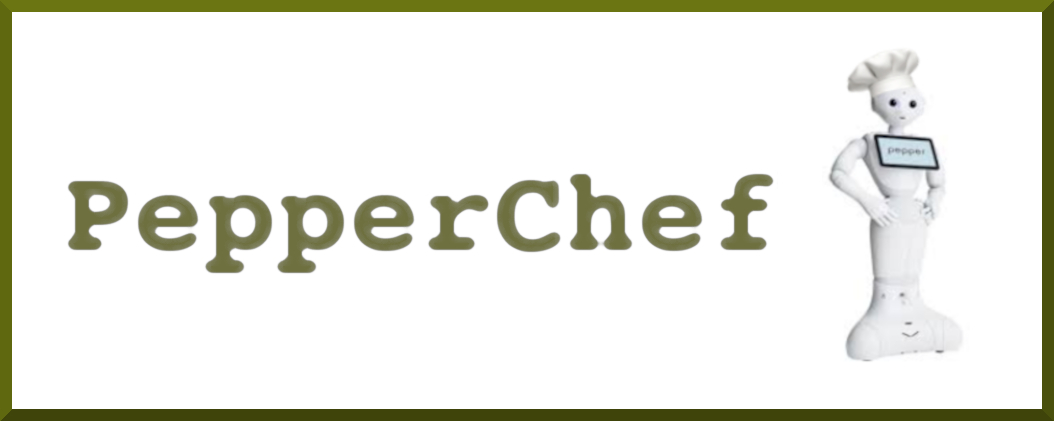
\includegraphics[width=0.4\textwidth]{pepperchef}
\caption{PepperChef logo}
\label{fig:comb}
\end{figure}

\section{Related Work}\label{cha:rel}

We are entering an era where robots are increasingly becoming a part of our lives. The thing we should cohabit with is that robots are not simple mechanical tools anymore. This new way of thinking has been very popular in the last years, thanks to the important growth of artificial intelligence and human-robot interaction sciences. Furthermore, there are high expectations for intelligent machines in the future. For these reasons, robots can't be considered just tools anymore. Our work, in fact, follows the arguments discussed in a commentary by Tony Prescott \cite{prescott} and tries to extend these thoughts in a real robot. This paper advances a criticism of the EPSRC principles of robotics and tries to reformulate them in a way in which robots are not considered just simple tools. As Prescott states in his work \textit{"the ontological status of robots might be best described as liminal—neither living nor simply mechanical"}. We can easily understand that consider a robot just as a tool is trivial, especially when people are able to create bonds with simpler products like chatbots, Tamagotchi, or voice assistants. This evidence is even more present in the HRI field, in which robot companions, for example, are highly requested from customers of all ages. We started our work carrying out this idea and trying to develop something more than just a tool. 

Recently, kitchen environments are getting more and more technological and complicated. I bet we everybody have at least three or four tools to use in different situations and for specific actions. Some other tools are capable of grouping more functionality, e.g. Kenwood and Bimby machines \footnote{(Thermomix) and Kenwood machines are domestic appliances offering various functions for cooking purposes.}. However, all of those kitchen tools are used to replace hand-made work and to obtain, most of the time, a better result. We can say that the use of these instruments has brought, of course, a great innovation. Anyway, nobody of those tools will ever ask you how your day is going or simply tell you what time is it. They won't even teach you how to cook some recipes and won't make you smile (most of the time they only make you angrier because of their complex use). But, most importantly, they will never stay with you and speak with you, and you will never have a friendship bond with them. For this reason, we introduce PepperChef. It won't be able to cook you an Italian risotto as a Kenwood machine may do, but it will, instead, teach you how to do it, making you enjoy the conversation and the time spent preparing the recipe. Resuming, we take into account the knowledge expansion of the final user while taking care of him through a companion robot that can dialogue and interact.  

In the development of any engineering project or application, the collection of data and its analysis for final evaluation is a really important step. This permits not only to understand how the system is performing but also a wide vision on the improvements that should be made to redesign the application. Once we reinforced and confirmed the message we wanted to convey and how the robot should have brought it, we made thought on how to analyze the effectiveness of Pepper and, more importantly, how people would have reacted to him. For this reason, we refer to a paper published by Bartneck et al. \cite{bartneck} ...

[papers  you have read that are related to your project (including the ones you presented, the ones mentioned during the lectures, etc.) and relation between these papers and your project]

\newpage
\section{Solution}\label{cha:sol}

PepperChef is meant to be run on a Pepper robot or an emulator of it. For this purpose, we took into consideration all the components of the robot provided by SoftBank robotics. Some of these, however, won't be used at all. This is due to our application development which is mainly focused in a simulated environment that, unfortunately, does not provide all the real services. Some examples are ....... . The communication process with the robot is mainly thought to be using real voice, making the process of communicating as natural as possible. Nevertheless, also the services for voice recognition and audio support are not available in the simulator, so we had to replace them with a chat channel. This is, fortunately, provided in the Android simulator. Users are able to speak with Pepper using the simulator chat and it will reply almost instantly in the same box. Pepper robot is also equipped with an Android tablet on its chest. We decided to highly use this component in our solution to make the dialog process more interactive and real. In fact, recipes preparation is more understandable is we can also look at it, more than listening to the procedures. The tablet plays an important role also with regard to the final user questionnaire for the evaluation of the robot. We can define the interaction with pepper a mixed one. It is always possible to speak (or chat in the simulator) with him while entering one of the tablet applications. Those applications running on the tablet are accessible by making an explicit request or replying affirmatively while talking with Pepper. Further details are shown in Section \ref{cha:res}. 

The advantage of interconnecting Pepper dialog with tablet apps is that the user will have a perception of semi-intelligence while talking with it. This makes the interaction more enjoyable and natural, like when a friend is showing you something on his smart-phone. PepperChef focuses its application also on touch-ability more than voice dialog and tablet entertainment. In fact, we added functionality in which Pepper is able to identify if someone is touching its head, asking the person if help is needed. This solution tries to make Pepper as confident as possible, trying not to scare people. In this way, we lay the foundations for a possible feeling of friendship and predict to have a more natural reaction from the final user.


[architecture of the solution: which components have been used, how they are connected each other, etc.]

\newpage
\section{Implementation}\label{cha:impl}

[details on the implementation, which libraries/tools you have used to implement the components, how do you put all together]

\newpage
\section{Results}\label{cha:res}

[description of some interactions, possibly commenting portion of the video, showing different modalities of interaction and different behaviors depending on different situations]

\newpage
\section{Conclusions}\label{cha:conc}

PepperChef, from our point of view, is a new kind of challenge. Many of the robotics systems take mainly into consideration the engineering part, both software, and mechanics, rather than the ethics and social part. That happens especially because most of the actual robots don't have to possess social functions, but have to, instead, carry out mechanical tasks independently or in collaboration with humans. The world of HRI (Human-Robot Interaction) was quite new to us and we explored the communication and social part of a robot more than the pure engineering aspects. We think that both the sides should be highly considered in designing a robot, also because of its presence in our society and the continuous contact with people. We enjoyed the time in developing PepperChef, especially when thinking that other people would have tested out its functionality, making it as much as possible appreciable and capable of understanding users' needs. As mentioned before, for the purpose of the project, we mixed the engineering part in developing the application with a thought of the possible social effects that the robot could have on people. The project was very stimulating and we believe it was a great experience to discover a new science, that of HRI.

Due to the Covid-19 emergency and, consequently, the strict access to the university, we weren't able to really try PepperChef. However, the simulator does a great job and the same virtual application could be, in the future, tested out on a real Pepper robot. Further work could be done collecting data from people and analyzing their opinion on the application and its functionality.  Another important step to increase the effectiveness of PepperChef is the one to focus on its gesturing, maybe executing actions and movements to better teach how to prepare a certain recipe. This was not easily verifiable on the Android simulator. Other important upgrades are the enlargement of the proposed recipes and a more complete questionnaire, taking into account other categories like anthropomorphism, animacy, and perceived safety. As mentioned in Chapter \ref{cha:sol}, those categories are not really analyzable in a simulator and we decided to omit them. However, the final questionnaire phase should remain short and not too heavy for the user, also to improve its compilation success.

\newpage
\section{References}
\begin{thebibliography}{999}

\bibitem{prescott}
	Tony J. Prescott, \emph{Robots are not just tools, Connection Science}, 29:2, 142-149, DOI: 10.1080/09540091.2017.1279125.

\bibitem{bartneck}
	Bartneck, C., Croft, E., \& Kulic, D., \emph{Measurement Instruments for the Anthropomorphism, Animacy, Likeability, Perceived Intelligence, and Perceived Safety of Robots}, International Journal of Social Robotics, 1(1), 71-81.

\bibitem{naoqi}
  \href{http://doc.aldebaran.com/2-5/dev/python/index.html}{NAOqi Software Development Kit for Python} (Link)  

\bibitem{naoqi2}
  \href{https://qisdk.softbankrobotics.com/sdk/doc/pepper-sdk/index.html}{NAOqi Software Development Kit for Android} (Link)  

\bibitem{hri}
	\href{https://bitbucket.org/iocchi/hri_software/src/master/}{HRI software with Docker support for NAOqi} (Link) 

\bibitem{modim}
	\href{https://bitbucket.org/mtlazaro/modim/src/master/}{Multi-mODal Interaction Manager for Pepper tablet} (Link)  

\end{thebibliography}

\end{document}


